%%%%%%%%%%%%%%%%%%%%%%%%%%%%%%%%%%%%%%%%%%%%%%%%%%%%%%%%%%%%%%%%%%%%%%%%%%%
%% This file is part of the book
%%
%% Algorithmic Graph Theory
%% http://code.google.com/p/graph-theory-algorithms-book/
%%
%% Copyright (C) 2010 David Joyner <wdjoyner@gmail.com>
%% Copyright (C) 2009, 2010, 2011 Minh Van Nguyen <nguyenminh2@gmail.com>
%%
%% See the file COPYING for copying conditions.
%%%%%%%%%%%%%%%%%%%%%%%%%%%%%%%%%%%%%%%%%%%%%%%%%%%%%%%%%%%%%%%%%%%%%%%%%%%

\chapter{Distance and Connectivity}
\label{chap:distance_connectivity}


%%%%%%%%%%%%%%%%%%%%%%%%%%%%%%%%%%%%%%%%%%%%%%%%%%%%%%%%%%%%%%%%%%%%%%%%%%%

\section{Paths and distance}


%%%%%%%%%%%%%%%%%%%%%%%%%%%%%%%%%%%%%%%%%%%%%%%%%%%%%%%%%%%%%%%%%%%%%%%%%%%

\subsection{Distance and metrics}

Consider an edge-weighted simple graph $G = (V,E,i,h)$ without
negative weight cycles. Here $E \subseteq V^{(2)}$, $i: E \to V^{(2)}$
is an incidence function as in~\eqref{eqn:introduction:edge_incidence},
which we regard as the identity function, and $h: E \to V$ is an
orientation function as in~\eqref{eqn:introduction:edge_orientation}.
Let $W: E \to \R$ be the weight function. (If $G$ is not provided with
a weight function on the edges, we assume that each edge has unit
weight.) If $v_1, v_2 \in V$ are two vertices and
$P = (e_1, e_2, \dots, e_m)$ is a $v_1$-$v_2$ path~(so $v_1$ is
incident to $e_1$ and $v_2$ is incident to $e_m$), define the
\emph{weight}\index{weight!path} of $P$ to be the sum of the weights
of the edges in $P$:
\[
W(P)
=
\sum_{i=1}^m W(e_i).
\]
The \emph{distance function}\index{distance!function}
$d: V \times V \to \R \cup \{\infty\}$ on $G$ is defined by
\[
d(v_1, v_2)
=
\infty
\]
if $v_1$ and $v_2$ lie in distinct connected components of $G$, and by
%%
\begin{equation}
\label{eqn:distance_connectivity:distance_as_minimum_path_weight}
d(v_1, v_2)
=
\min_P W(P)
\end{equation}
%%
otherwise, where the minimum is taken over all paths $P$ from $v_1$ to
$v_2$. By hypothesis, $G$ has no negative weight cycles so the minimum
in~\eqref{eqn:distance_connectivity:distance_as_minimum_path_weight}
exists. It follows by definition of the distance function that
$d(u,v) = \infty$ if and only if there is no path between $u$ and $v$.

How we interpret the distance function $d$ depends on the meaning of
the weight function $W$. In practical applications, vertices can
represent physical locations such as cities, sea ports, or
landmarks. An edge weight could be interpreted as the physical
distance in kilometers between two cities, the monetary cost of
shipping goods from one sea port to another, or the time required to
travel from one landmark to another. Then $d(u,v)$ could mean the
shortest route in kilometers between two cities, the lowest cost
incurred in transporting goods from one sea port to another, or the
least time required to travel from one landmark to another.

The distance function\index{distance!function} $d$ is not in general a
metric\index{metric}, i.e. the triangle
inequality\index{triangle inequality} does not in general hold for
$d$. However, when the distance function is a metric then $G$ is
called a \emph{metric graph}\index{metric graph}. The theory of
metric\index{metric graph} graphs, due to their close connection with
tropical curves, is an active area of research. For more information
on metric graphs, see Baker\index{Baker, Matthew} and
Faber\index{Faber, Xander}~\cite{BakerFaber2006}.


%%%%%%%%%%%%%%%%%%%%%%%%%%%%%%%%%%%%%%%%%%%%%%%%%%%%%%%%%%%%%%%%%%%%%%%%%%%

\subsection{Radius and diameter}

A new hospital is to be built in a large city. Construction has not
yet started and a number of urban planners are discussing the future
location of the new hospital. What is a possible location for the new
hospital and how are we to determine this location? This is an example
of a class of problems known as facility location problems. Suppose
our objective in selecting a location for the hospital is to minimize
the maximum response time between the new hospital and the site of an
emergency. To help with our decision making, we could use the notion
of the center of a graph.

The center of a graph $G = (V,E)$ is defined in terms of the
eccentricity of the graph under consideration. The
\emph{eccentricity}\index{eccentricity}
$\epsilon: V \to \R$\index{$\epsilon$} is defined as follows. For any
vertex $v$, the eccentricity $\epsilon(v)$ is the greatest distance
between $v$ and any other vertex in $G$. In symbols, the eccentricity
is expressible as
\[
\epsilon(v)
=
\max_{u \in V} d(u,v).
\]
For example, in a tree $T$ with root $r$ the eccentricity of $r$ is
the height of $T$. In the graph of
Figure~\ref{fig:distance_connectivity:find_eccentricity_center_radius_diameter},
the eccentricity of $2$ is $5$ and the shortest paths that yield
$\epsilon(2)$ are
%%
\begin{align*}
P_1: 2, 3, 4, 14, 15, 16 \\
P_2: 2, 3, 4, 14, 15, 17.
\end{align*}
%%
The eccentricity of a vertex $v$ can be thought of as an upper bound
on the distance from $v$ to any other vertex in $G$. Furthermore, we
have at least one vertex in $G$ whose distance from $v$ is
$\epsilon(v)$.

\begin{figure}[!htbp]
\centering
%%%%%%%%%%%%%%%%%%%%%%%%%%%%%%%%%%%%%%%%%%%%%%%%%%%%%%%%%%%%%%%%%%%%%%%%%%%
%% This file is part of the book
%%
%% Algorithmic Graph Theory
%% http://code.google.com/p/graph-theory-algorithms-book/
%%
%% Copyright (C) 2009--2011 Minh Van Nguyen <nguyenminh2@gmail.com>
%%
%% See the file COPYING for copying conditions.
%%%%%%%%%%%%%%%%%%%%%%%%%%%%%%%%%%%%%%%%%%%%%%%%%%%%%%%%%%%%%%%%%%%%%%%%%%%

\documentclass{article}

\usepackage{tikz}
\usetikzlibrary{external}
\tikzexternalize{determine-eccentricity-radius-diameter}

\begin{document}

\begin{figure}
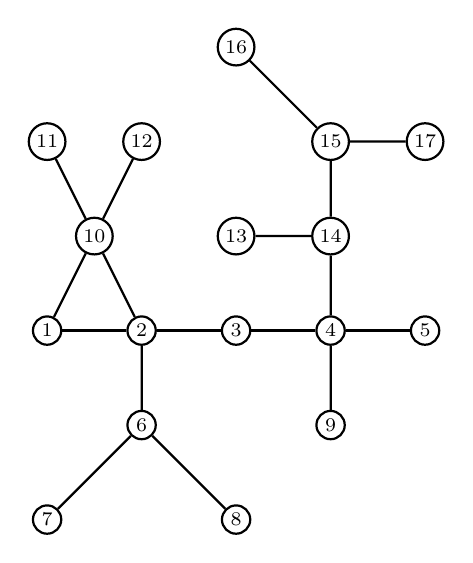
\begin{tikzpicture}
[lineDecorate/.style={-,thick},%
  nodeDecorate/.style={shape=circle,inner sep=1.5pt,draw,thick},%
  scale=1.2]
\scriptsize
%% nodes or vertices
\foreach \nodename/\x/\y in {
  1/1/0, 2/2/0, 3/3/0, 4/4/0, 5/5/0, 6/2/-1, 7/1/-2, 8/3/-2, 9/4/-1,
  10/1.5/1, 11/1/2, 12/2/2, 13/3/1, 14/4/1, 15/4/2, 16/3/3, 17/5/2}
{
  \node (\nodename) at (\x,\y) [nodeDecorate] {$\nodename$};
}
%% edges or lines
\path
\foreach \startnode/\endnode in {
  1/2, 1/10, 2/3, 2/6, 2/10, 3/4, 4/5, 4/9, 4/14, 6/7, 6/8, 10/11,
  10/12, 13/14, 14/15, 15/16, 15/17}
{
  (\startnode) edge[lineDecorate] node {} (\endnode)
};
\end{tikzpicture}
\end{figure}

\end{document}

\caption{Determine the eccentricity, center, radius, and diameter.}
\label{fig:distance_connectivity:find_eccentricity_center_radius_diameter}
\end{figure}

\begin{table}[!htbp]
\centering
%%%%%%%%%%%%%%%%%%%%%%%%%%%%%%%%%%%%%%%%%%%%%%%%%%%%%%%%%%%%%%%%%%%%%%%%%%%
%% This file is part of the book
%%
%% Algorithmic Graph Theory
%% http://code.google.com/p/graph-theory-algorithms-book/
%%
%% Copyright (C) 2009--2011 Minh Van Nguyen <nguyenminh2@gmail.com>
%%
%% See the file COPYING for copying conditions.
%%%%%%%%%%%%%%%%%%%%%%%%%%%%%%%%%%%%%%%%%%%%%%%%%%%%%%%%%%%%%%%%%%%%%%%%%%%

\begin{tabular}{r|ccccccccccccccccc}
$v$ & $1$ & $2$ & $3$ & $4$ & $5$ & $6$ & $7$ & $8$ & $9$ & $10$ & $11$ & $12$ & $13$ & $14$ & $15$ & $16$ & $17$ \\\hline
$\epsilon(v)$ & $6$ & $5$ & $4$ & $4$ & $5$ & $6$ & $7$ & $7$ & $5$ & $6$ & $7$ & $7$ & $6$ & $5$ & $6$ & $7$ & $7$
\end{tabular}

\caption{Eccentricity distribution.}
\label{tab:distance_connectivity:eccentricity_distribution}
\end{table}

To motivate the notion of the radius of a graph, consider the
distribution of eccentricity among vertices of the graph $G$ in
Figure~\ref{fig:distance_connectivity:find_eccentricity_center_radius_diameter}.
The required eccentricity distribution is shown in
Table~\ref{tab:distance_connectivity:eccentricity_distribution}. Among
the eccentricities in the latter table, the minimum eccentricity is
$\epsilon(3) = \epsilon(4) = 4$. An intuitive interpretation is that
both of the vertices $3$ and $4$ have the shortest distance to any
other vertices in $G$. We can invoke an analogy with plane geometry as
follows. If a circle has radius $r$, then the distance from the center
of the circle to any point within the circle is at most $r$. The
minimum eccentricity in graph theory plays a role similar to the
radius of a circle. If an object is strategically
positioned---e.g. a vertex with minimum eccentricity or the center of
a circle---then its greatest distance to any other object is
guaranteed to be minimum. With the above analogy in mind, we define
the \emph{radius} of a graph $G = (V,E)$, written
$\radius(G)$\index{$\radius(G)$}, to be the minimum eccentricity among
the eccentricity distribution of $G$. In symbols,
\[
\radius(G)
=
\min_{v \in V} \epsilon(v).
\]
The \emph{center} of $G$, written $C(G)$, is the set of vertices with
minimum eccentricity. Thus the graph in
Figure~\ref{fig:distance_connectivity:find_eccentricity_center_radius_diameter}
has radius $4$ and center $\{3, 4\}$. As should be clear from the
latter example, the radius is a number whereas the center is a
set. Refer to the beginning of the section where we mentioned the
problem of selecting a location for a new hospital. We could use a
graph to represent the geography of the city wherein the hospital is
to be situated and select a location that is in the center of the
graph.

Consider now the maximum eccentricity of a
graph. In~\eqref{eqn:graph_algorithms:graph_diameter} we defined the
\emph{diameter} of a graph $G = (V,E)$ by
\[
\diam(G)\index{$\diam(G)$}
=
\max_{\substack{u,v \in V \\ u \neq v}} d(u,v).
\]
The diameter of $G$ can also be defined as the maximum eccentricity of
any vertex in $G$:
\[
\diam(G)
=
\max_{v \in V} \epsilon(v).
\]
In case $G$ is disconnected, define its diameter to be
$\diam(G) = \infty$. To compute $\diam(G)$, use the Floyd-Roy-Warshall
algorithm~(see
section~\ref{sec:graph_algorithms:Floyd_Roy_Warshall_algorithm}) to
compute the shortest distance between each pair of vertices. The
maximum of these distances is the diameter. The set of vertices of $G$
with maximum eccentricity is called the \emph{periphery} of $G$,
written $\per(G)$\index{$\per(G)$}. The graph in
Figure~\ref{fig:distance_connectivity:find_eccentricity_center_radius_diameter}
has diameter $7$ and periphery $\{7, 8, 11, 12, 16, 17\}$.

\begin{theorem}
\textbf{Eccentricities of adjacent vertices.}
Let $G = (V,E)$ be an undirected, connected graph having nonnegative
edge weights. If $uv \in E$ and $W$ is a weight function for $G$, then
$|\epsilon(u) - \epsilon(v)| \leq W(uv)$.
\end{theorem}

\begin{proof}
By definition, we have $d(u,x) \leq \epsilon(u)$ and
$d(v,x) \leq \epsilon(v)$ for all $x \in V$. Let $w \in V$ such that
$d(u,w) = \epsilon(u)$. Apply the triangle inequality to obtain
%%
\begin{align*}
d(u,w) &\leq d(u,v) + d(v,w) \\
\epsilon(u) &\leq W(uv) + d(v,w) \\
            &\leq W(uv) + \epsilon(v)
\end{align*}
%%
from which we have $\epsilon(u) - \epsilon(v) \leq W(uv)$. Repeating
the above argument with the role of $u$ and $v$ interchanged yields
$\epsilon(v) - \epsilon(u) \leq W(uv)$. Both
$\epsilon(u) - \epsilon(v) \leq W(uv)$ and
$\epsilon(v) - \epsilon(u) \leq W(uv)$ together yields the inequality
$|\epsilon(u) - \epsilon(v)| \leq W(uv)$ as required.
\end{proof}


%%%%%%%%%%%%%%%%%%%%%%%%%%%%%%%%%%%%%%%%%%%%%%%%%%%%%%%%%%%%%%%%%%%%%%%%%%%

\subsection{Center of trees}

Given a tree $T$ of order $\geq 3$, we want to derive a bound on the
number of vertices that comprise the center of $T$. A graph in general
can have one, two, or more number of vertices for its center. Indeed,
for any integer $n > 0$ we can construct a graph whose center has
cardinality $n$. The cases for $n = 1, 2, 3$ are illustrated in
Figure~\ref{fig:distance_connectivity:graphs_arbitrarily_large_centers}. But
can we do the same for trees? That is, given any positive integer $n$
does there exist a tree whose center has $n$ vertices? It turns out
that the center of a tree cannot have more than two vertices, a result
first discovered~\cite{Jordan1869} by Camille
Jordan\index{Jordan, Camille} in~1869.

\begin{figure}[!htbp]
\centering
%%%%%%%%%%%%%%%%%%%%%%%%%%%%%%%%%%%%%%%%%%%%%%%%%%%%%%%%%%%%%%%%%%%%%%%%%%%
%% This file is part of the book
%%
%% Algorithmic Graph Theory
%% http://code.google.com/p/graph-theory-algorithms-book/
%%
%% Copyright (C) 2009, 2010, 2011 Minh Van Nguyen <nguyenminh2@gmail.com>
%%
%% See the file COPYING for copying conditions.
%%%%%%%%%%%%%%%%%%%%%%%%%%%%%%%%%%%%%%%%%%%%%%%%%%%%%%%%%%%%%%%%%%%%%%%%%%%

\documentclass{article}

\usepackage{subfigure}
\usepackage{tikz}
\usetikzlibrary{external}
\tikzexternalize{arbitrarily-large-center}

\begin{document}

\begin{figure}
\subfigure[$|C(G)| = 1$]{
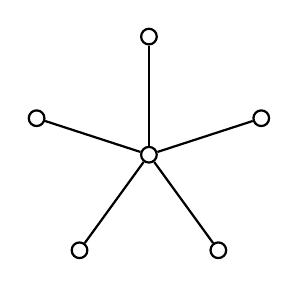
\begin{tikzpicture}
[nodeDecorate/.style={shape=circle,inner sep=2pt,draw,thick},%
  lineDecorate/.style={-,thick},%
  scale=1.5]
%% complete bipartite graph K_{1,5}
%% nodes or vertices
\foreach \nodename/\x/\y in {
  1/0.9510/0.3090, 2/0/1, 3/-0.9510/0.3090, 4/-0.5877/-0.8090,
  5/0.5877/-0.8090, 6/0/0}
{
  \node (\nodename) at (\x,\y) [nodeDecorate] {};
}
%% edges or lines
\path
\foreach \startnode/\endnode in {1/6, 2/6, 3/6, 4/6, 5/6}
{
  (\startnode) edge[lineDecorate] node {} (\endnode)
};
\end{tikzpicture}
}
%%
%%
\qquad
\subfigure[$|C(G)| = 2$]{
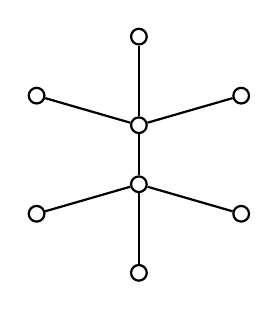
\begin{tikzpicture}
[nodedecorate/.style={shape=circle,inner sep=2pt,draw,thick},%
  linedecorate/.style={-,thick},%
  scale=1.5]
%% nodes or vertices
\foreach \nodename/\x/\y in {1/0.8660/0.5, 2/0/1, 3/-0.8660/0.5,
  4/-0.8660/-0.5, 5/0/-1, 6/0.8660/-0.5, 7/0/0.25, 8/0/-0.25}
{
  \node (\nodename) at (\x,\y) [nodedecorate] {};
}
%% edges or lines
\path
\foreach \startnode/\endnode in {7/1, 7/2, 7/3, 7/8, 8/4, 8/5, 8/6}
{
  (\startnode) edge[linedecorate] node {} (\endnode)
};
\end{tikzpicture}
}
%%
%%
\qquad
\subfigure[$|C(G)| = 3$]{
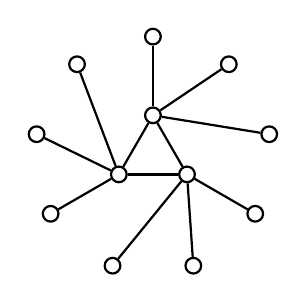
\begin{tikzpicture}
[nodedecorate/.style={shape=circle,inner sep=2pt,draw,thick},%
  linedecorate/.style={-,thick},%
  scale=1.5]
%% nodes or vertices
\foreach \nodename/\x/\y in {
  %% outer vertices
  1/0/1, 2/0.6427/0.7660, 3/0.9848/0.1736, 4/0.8660/-0.5,
  5/0.3420/-0.9396, 6/-0.3420/-0.9396, 7/-0.8660/-0.5,
  8/-0.9848/0.1736, 9/-0.6427/0.7660,
  %% inner vertices
  10/0/0.3333, 11/0.2886/-0.1666, 12/-0.2886/-0.1666}
{
  \node (\nodename) at (\x,\y) [nodedecorate] {};
}
%% edges or lines
\path
\foreach \startnode/\endnode in {
  10/1, 10/2, 10/3, 11/4, 11/5, 11/6, 12/7, 12/8, 12/9, 10/11, 11/12, 12/10}
{
  (\startnode) edge[linedecorate] node {} (\endnode)
};
\end{tikzpicture}
}
\end{figure}

\end{document}

\caption{Constructing graphs with arbitrarily large centers.}
\label{fig:distance_connectivity:graphs_arbitrarily_large_centers}
\end{figure}

\begin{theorem}
\textbf{Jordan~\cite{Jordan1869}.}
If a tree $T$ has order $\geq 3$, then the center of $T$ is either a
single vertex or two adjacent vertices.
\end{theorem}

\begin{proof}
As all eccentric vertices of $T$ are leaves~(see
problem~\ref{chap:distance_connectivity}.\ref{prob:distance_connectivity:eccentric_vertices_laves}),
removing all the leaves of $T$ decreases the eccentricities of the
remaining vertices by one. The tree comprised of the surviving
vertices has the same center as $T$. Continue pruning leaves as
described above and note that the tree comprised of the surviving
vertices has the same center as the previous tree. After a finite
number of leaf pruning stages, we eventually end up with a tree made
up of either one vertex or two adjacent vertices. The vertex set of
this final tree is the center of $T$.
\end{proof}


%%%%%%%%%%%%%%%%%%%%%%%%%%%%%%%%%%%%%%%%%%%%%%%%%%%%%%%%%%%%%%%%%%%%%%%%%%%

\subsection{Distance matrix}

In sections~\ref{sec:introduction:distance_matrix}
and~\ref{sec:graph_algorithms:weights_distances}, the distance matrix
$D$ of a graph $G$ was defined to be $D = [d_{ij}]$, where
$d_{ij} = d(v_i, v_j)$ and the vertices of $G$ are indexed by
$V = \{v_0, v_1, \dots, v_k\}$. The matrix $D$ is square where we set
$d_{ij} = 0$ for entries along the main diagonal. If there is no path
from $v_i$ to $v_j$, then we set $d_{ij} = \infty$. If $G$ is
undirected, then $D$ is symmetric and is equal to its transpose,
i.e. $D^T = D$. To compute the distance matrix $D$, apply the
Floyd-Roy-Warshall\index{Floyd-Roy-Warshall algorithm} algorithm to
determine the distances between all pairs of vertices. Refer to
Figure~\ref{fig:distance_connectivity:distance_matrix_directed_undirected_graphs}
for examples of distance matrices of directed and undirected
graphs. In the remainder of this section, ``graph'' refers to an
undirected graph unless otherwise specified.

\begin{figure}[!htbp]
\centering
\index{matrix!distance}
%%%%%%%%%%%%%%%%%%%%%%%%%%%%%%%%%%%%%%%%%%%%%%%%%%%%%%%%%%%%%%%%%%%%%%%%%%%
%% This file is part of the book
%%
%% Algorithmic Graph Theory
%% http://code.google.com/p/graph-theory-algorithms-book/
%%
%% Copyright (C) 2009, 2010, 2011 Minh Van Nguyen <nguyenminh2@gmail.com>
%%
%% See the file COPYING for copying conditions.
%%%%%%%%%%%%%%%%%%%%%%%%%%%%%%%%%%%%%%%%%%%%%%%%%%%%%%%%%%%%%%%%%%%%%%%%%%%

%% digraph
\subfigure[]{
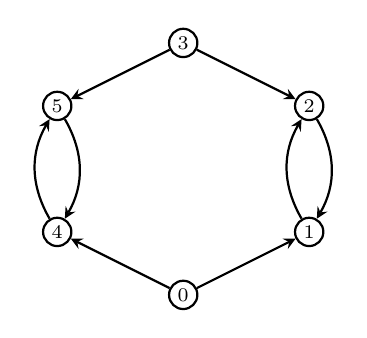
\begin{tikzpicture}
[arrowDecorate/.style={->,>=stealth,thick},%
  nodeDecorate/.style={shape=circle,inner sep=1.5pt,draw,thick},%
  scale=0.8]
\scriptsize
%% nodes or vertices
\foreach \nodename/\x/\y in {1/2/1, 2/2/3, 3/0/4, 0/0/0, 4/-2/1, 5/-2/3}
{
  \node (\nodename) at (\x,\y) [nodeDecorate] {$\nodename$};
}
%% edges or lines
\path
(1) edge[arrowDecorate,bend left] node {} (2)
(2) edge[arrowDecorate,bend left] node {} (1)
(3) edge[arrowDecorate] node {} (2)
(3) edge[arrowDecorate] node {} (5)
(0) edge[arrowDecorate] node {} (1)
(0) edge[arrowDecorate] node {} (4)
(4) edge[arrowDecorate,bend left] node {} (5)
(5) edge[arrowDecorate,bend left] node {} (4);
\end{tikzpicture}
%%
%%
\qquad\qquad
%%
%%
\begin{tikzpicture}
\node at (0,0) {%
$
\begin{bmatrix}
0      & 1      & 2      & \infty & 1      & 2 \\
\infty & 0      & 1      & \infty & \infty & \infty \\
\infty & 1      & 0      & \infty & \infty & \infty \\
\infty & 2      & 1      & 0      & 2      & 1 \\
\infty & \infty & \infty & \infty & 0      & 1 \\
\infty & \infty & \infty & \infty & 1      & 0
\end{bmatrix}
$
};
\end{tikzpicture}
}
%%
%%
\qquad
%% graph
\subfigure[]{
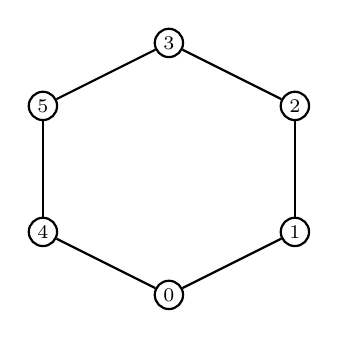
\begin{tikzpicture}
[lineDecorate/.style={-,thick},%
  nodeDecorate/.style={shape=circle,inner sep=1.5pt,draw,thick},%
  scale=0.8]
\scriptsize
%% nodes or vertices
\foreach \nodename/\x/\y in {1/2/1, 2/2/3, 3/0/4, 0/0/0, 4/-2/1, 5/-2/3}
{
  \node (\nodename) at (\x,\y) [nodeDecorate] {$\nodename$};
}
%% edges or lines
\path
\foreach \startnode/\endnode in {1/2, 1/0, 2/3, 3/5, 0/4, 4/5}
{
  (\startnode) edge[lineDecorate] node {} (\endnode)
};
\end{tikzpicture}
%%
%%
\qquad\qquad
%%
%%
\begin{tikzpicture}
\node at (0,0) {%
$
\begin{bmatrix}
0 & 1 & 2 & 3 & 1 & 2 \\
1 & 0 & 1 & 2 & 2 & 3 \\
2 & 1 & 0 & 1 & 3 & 2 \\
3 & 2 & 1 & 0 & 2 & 1 \\
1 & 2 & 3 & 2 & 0 & 1 \\
2 & 3 & 2 & 1 & 1 & 0
\end{bmatrix}
$
};
\end{tikzpicture}
}

\caption{Distance matrices of directed and undirected graphs.}
\label{fig:distance_connectivity:distance_matrix_directed_undirected_graphs}
\end{figure}

Instead of one distance matrix, we can define several distance
matrices on $G$. Consider an edge-weighted graph $G = (V,E)$ without
negative weight cycles and let
\[
d: V \times V \to \R \cup \{\infty\}
\]
be a distance function of $G$. Let $\partial = \diam(G)$ be the
diameter of $G$ and index the vertices of $G$ in some arbitrary but
fixed manner, say $V = \{v_0, v_1, \dots, v_n\}$. The sequence of
\emph{distance matrices}\index{matrix!distance} of $G$ are a sequence
of $(n - 1) \times (n - 1)$ matrices $A_1, A_2, \dots, A_\partial$ where
\[
(A_k)_{ij}
=
\begin{cases}
1, & \text{if $d(v_i, v_j) = k$}, \\
0, & \text{otherwise}.
\end{cases}
\]
In particular, $A_1$ is the usual adjacency matrix $A$. To compute the
sequence of distance matrices of $G$, use the
Floyd-Roy-Warshall\index{Floyd-Roy-Warshall algorithm} algorithm to
compute the distance between each pair of vertices and assign the
resulting distance to the corresponding matrix $A_i$.

The distance matrix arises in several applications, including
communication network design~\cite{GrahamPollak1971} and network flow
algorithms~\cite{Dijkstra1959}. Thanks to Graham\index{Graham, R. L.}
and Pollak\index{Pollak, O.}~\cite{GrahamPollak1971}, the following
unusual fact is known. If $T$ is any tree then
\[
\det D(T)
=
(-1)^{n - 1} (n - 1) 2^{n - 2}
\]
where $n$ denotes the order of $T$. In particular, the determinant of
the distance matrix of a tree is independent of the structure of the
tree.  This fact is proven in the paper~\cite{GrahamPollak1971}, but
see also~\cite{EdelbergEtAl1976}.


%%%%%%%%%%%%%%%%%%%%%%%%%%%%%%%%%%%%%%%%%%%%%%%%%%%%%%%%%%%%%%%%%%%%%%%%%%%

\section{Vertex and edge connectivity}

If $G = (V,E)$ is a graph and $U \subseteq V$ is a vertex set with the
property that $G - U$ has more connected components than $G$, then we
call $U$ a \emph{vertex-cut}\index{vertex-cut}. The term
\emph{cut-vertex}\index{cut-vertex} or
\emph{cut-point}\index{cut-point} is used when the vertex-cut consists
of exactly one vertex. For an intuitive appreciation of vertex-cut,
suppose $G = (V,E)$ is a connected graph. Then $U \subseteq V$ is a
vertex-cut if the vertex\index{vertex!deletion subgraph} deletion
subgraph $G - U$ is disconnected. For example, the cut-vertex of the
graph in Figure~\ref{fig:distance_connectivity:claw_graph} is the
vertex $0$. By $\kappa_v(G)$\index{$\kappa_v(G)$} we mean the
\emph{vertex connectivity}\index{vertex connectivity} of a connected
graph $G$, defined as the minimum number of vertices whose removal
would either disconnect $G$ or reduce $G$ to the trivial graph. The
vertex connectivity $\kappa_v(G)$ is also written as
$\kappa(G)$\index{$\kappa(G)$}. The vertex connectivity of the graph
in Figure~\ref{fig:distance_connectivity:claw_graph} is
$\kappa_v(G) = 1$ because we only need to remove vertex $0$ in order
to disconnect the graph. The vertex connectivity of a connected graph
$G$ is thus the vertex-cut of minimum cardinality. And $G$ is said to
be $k$-\emph{connected}\index{$k$-connected} if $\kappa_v(G) \geq k$.
From the latter definition, it immediately follows that if $G$ has at
least $3$ vertices and is $k$-connected then any vertex-cut of $G$ has
at least cardinality $k$. For instance, the graph in
Figure~\ref{fig:distance_connectivity:claw_graph} is $1$-connected. In
other words, $G$ is $k$-connected if the graph remains connected even
after removing any $k - 1$ or fewer vertices from $G$.

\begin{figure}[!htbp]
\centering
\index{cut-edge}
\index{cut-vertex}
\index{claw graph}
%%%%%%%%%%%%%%%%%%%%%%%%%%%%%%%%%%%%%%%%%%%%%%%%%%%%%%%%%%%%%%%%%%%%%%%%%%%
%% This file is part of the book
%%
%% Algorithmic Graph Theory
%% http://code.google.com/p/graph-theory-algorithms-book/
%%
%% Copyright (C) 2009, 2010, 2011 Minh Van Nguyen <nguyenminh2@gmail.com>
%%
%% See the file COPYING for copying conditions.
%%%%%%%%%%%%%%%%%%%%%%%%%%%%%%%%%%%%%%%%%%%%%%%%%%%%%%%%%%%%%%%%%%%%%%%%%%%

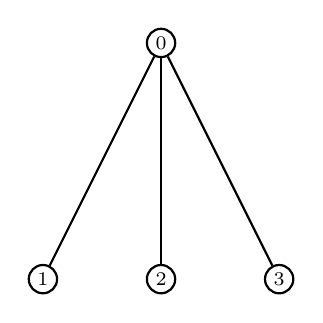
\begin{tikzpicture}
[nodeDecorate/.style={shape=circle,inner sep=1.5pt,draw,thick},%
  lineDecorate/.style={-,thick},%
  scale=1.5]
\scriptsize
%% nodes or vertices
\foreach \nodename/\x/\y in {1/0/0, 2/1/0, 3/2/0, 0/1/2}
{
  \node (\nodename) at (\x,\y) [nodeDecorate] {$\nodename$};
}
%% edges or lines
\path
\foreach \startnode/\endnode in {0/1, 0/2, 0/3} {
  (\startnode) edge[lineDecorate] node {} (\endnode)
};
\end{tikzpicture}

\caption{A claw graph with $4$ vertices.}
\label{fig:distance_connectivity:claw_graph}
\end{figure}

\begin{figure}[!htbp]
\centering
\index{Petersen graph}
%%%%%%%%%%%%%%%%%%%%%%%%%%%%%%%%%%%%%%%%%%%%%%%%%%%%%%%%%%%%%%%%%%%%%%%%%%%
%% This file is part of the book
%%
%% Algorithmic Graph Theory
%% http://code.google.com/p/graph-theory-algorithms-book/
%%
%% Copyright (C) 2009, 2010, 2011 Minh Van Nguyen <nguyenminh2@gmail.com>
%%
%% See the file COPYING for copying conditions.
%%%%%%%%%%%%%%%%%%%%%%%%%%%%%%%%%%%%%%%%%%%%%%%%%%%%%%%%%%%%%%%%%%%%%%%%%%%

\documentclass{article}

\usepackage{tikz}
\usetikzlibrary{external}
\tikzexternalize{petersen-graph}

\begin{document}

\begin{figure}
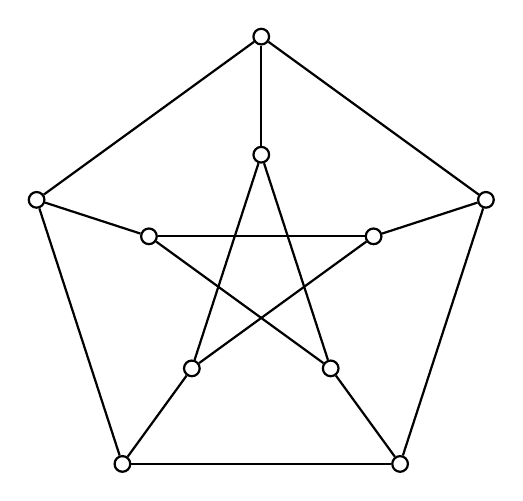
\begin{tikzpicture}
[nodeDecorate/.style={shape=circle,inner sep=2pt,draw,thick},%
  lineDecorate/.style={-,thick},scale=1.5]
%% nodes or vertices
\foreach \nodename/\x/\y in {
  %% outer pentagon
  0/0/2, 1/-1.9021/0.6180, 2/-1.1755/-1.6180, 3/1.1755/-1.6180,
  4/1.9021/0.6180,
  %% inner pentagon
  5/0/1, 6/-0.9510/0.3090, 7/-0.5877/-0.8090, 8/0.5877/-0.8090,
  9/0.9510/0.3090}
{
  \node (\nodename) at (\x,\y) [nodeDecorate] {};
}
%% edges or lines
\path
\foreach \startnode/\endnode in {0/1, 0/4, 0/5, 1/2, 1/6, 2/3, 2/7,
  3/4, 3/8, 4/9, 5/7, 5/8, 6/8, 6/9, 7/9}
{
  (\startnode) edge[lineDecorate] node {} (\endnode)
};
\end{tikzpicture}
\end{figure}

\end{document}

\caption{The Petersen graph on $10$ vertices.}
\label{fig:distance_connectivity:petersen_graph}
\end{figure}

\begin{example}
\rm
Here is a Sage example concerning $\kappa(G)$ using the
Petersen\index{Petersen graph} graph depicted in
Figure~\ref{fig:distance_connectivity:petersen_graph}. A linear
programming Sage package, such as GLPK, must be installed for the
commands below to work.
%%
\begin{lstlisting}
sage: G = graphs.PetersenGraph()
sage: len(G.vertices())
10
sage: G.vertex_connectivity()
3.0
sage: G.delete_vertex(0)
sage: len(G.vertices())
9
sage: G.vertex_connectivity()
2.0
\end{lstlisting}
\qed
\end{example}

The notions of edge-cut and cut-edge are similarly defined. Let
$G = (V,E)$ be a graph and $D \subseteq E$ an edge set such that the
edge deletion subgraph $G - D$ has more components than $G$. Then $D$
is called an \emph{edge-cut}\index{edge-cut}. An edge-cut $D$ is said
to be \emph{minimal} if no proper subset of $D$ is an edge-cut. The
term \emph{cut-edge}\index{cut-edge} or \emph{bridge}\index{bridge} is
reserved for the case where the set $D$ is a singleton. Think of a
cut-edge as an edge whose removal from a connected graph would result
in that graph being disconnected. Going back to the case of the graph
in Figure~\ref{fig:distance_connectivity:claw_graph}, each edge of the
graph is a cut-edge. The \emph{edge connectivity} of a connected graph
$G$, written $\kappa_e(G)$\index{$\kappa_e(G)$} and sometimes denoted
by $\lambda(G)$\index{$\lambda(G)$}, is the minimum number of edges
whose removal would disconnect $G$. In other words, $\kappa_e(G)$ is
the minimum cardinality among all edge-cuts of $G$. Furthermore, $G$
is said to be $k$-\emph{edge-connected}\index{$k$-edge-connected} if
$\kappa_e(G) \geq k$. A connected graph that is $k$-edge-connected is
guaranteed to be connected after removing $\leq k - 1$ edges from
it. When we have removed $k$ or more edges, then the graph would
become disconnected. The graph in
Figure~\ref{fig:distance_connectivity:claw_graph} has edge
connectivity $\kappa_e(G) = 1$ and is $1$-edge-connected.

Vertex and edge connectivity are intimately related to the reliability
and survivability of computer networks. If a computer network
$G$~(which is a connected graph) is $k$-connected, then it would
remain connected despite the failure of at most $k - 1$ network
nodes. Similarly, $G$ is $k$-edge-connected if the network remains
connected after the failure of at most $k - 1$ network links. In
practical terms, a network with redundant nodes and/or links can
afford to endure the failure of a number of nodes and/or links and
still be connected, whereas a network with very few redundant nodes
and/or links~(e.g. something close to a spanning tree) is more prone
to be disconnected. A $k$-connected or $k$-edge-connected network is
more robust (i.e. can withstand) against node and/or link failures
than is a $j$-connected or $j$-edge-connected network, where $j < k$.

\begin{proposition}
If $\delta(G)$ is the minimum degree of an undirected connected graph
$G$, then the edge connectivity of $G$ satisfies
$\kappa_e(G) \leq \delta(G)$.
\end{proposition}

\begin{proof}
Choose a vertex $v \in V(G)$ whose degree is
$\deg(v) = \delta(G)$. Deleting the $\delta(G)$ edges incident on $v$
suffices to separate $v$ from the remaining vertices of $G$.
\end{proof}

Let $G = (V,E)$ be a graph and suppose $X_1$ and $X_2$ comprise a
partition of $V$. A \emph{partition-cut} of $G$, denoted
$\langle X_1, X_2 \rangle$, is the set of all edges of $G$ with one
endpoint in $X_1$ and the other endpoint in $X_2$. If $G$ is a
bipartite graph with bipartition $X_1$ and $X_2$, then
$\langle X_1, X_2 \rangle$ is a partition-cut of $G$. It follows that
a partition-cut is also an edge-cut.

\begin{proposition}
An undirected connected graph $G$ is $k$-edge-connected if and only if
any partition-cut of $G$ has at least $k$ edges.
\end{proposition}

\begin{proof}
Assume that $G$ is $k$-edge-connected. Then each edge-cut has at least
$k$ edges. As a partition-cut is an edge-cut, then any partition-cut
of $G$ has at least $k$ edges.

On the other hand, suppose each partition-cut has at least $k$
edges. If $D$ is a minimal edge-cut of $G$ and $X_1$ and $X_2$ are the
vertex sets of the two components of $G - D$, then
$D = \langle X_1, X_2 \rangle$. To see this, note that
$D \subseteq \langle X_1, X_2 \rangle$. If
$\langle X_1, X_2 \rangle - D \neq \emptyset$ then choose some
$e \in \langle X_1, X_2 \rangle$ such that $e \notin D$. The endpoints
of $e$ belong to the same component of $G - D$, in contradiction of
the definition of $X_1$ and $X_2$. Thus any minimal edge-cut is a
partition-cut and conclude that any edge-cut has at least $k$ edges.
\end{proof}

%% NOTE: need to polish up statement and proof of Bondy's theorem.
%% \begin{theorem}
%% (Bondy's theorem)
%% {\rm
%% Suppose

%% \begin{itemize}
%% \item
%% $G=(V,E)$ is a connected simple graph with $n=|V|$,
%% \item
%% $0<k<n$,
%% \item
%% the (non-decreasing) degree sequence
%% $[d_1,d_2,\dots, d_n]$ satisfies
%% $d_j\geq j+k-1$, for $1\leq j\leq n-1-d_{n-k+1}$,
%% \end{itemize}
%% then $G$ is $k$-vertex-connected.
%% }
%% \end{theorem}
%% \index{Bondy's theorem}

%% \begin{proof}[Solution]
%% Suppose not, so $\kappa(G)<k$. Then there exists an
%% $S\subset V$, $|S|=s<k$, such that $G'=G-S$ has more
%% than one connected component. Let $H$ be connected
%% component of $G'$ of minimal number of
%% vertices, $j=V(H)$. If $v\in V(H)$ then
%% $\deg_G(v)\leq j-1+s$, since $v$ is not adjacent to any
%% vertex in any other connected component of $G'$.

%% Since $H$ was chosen minimally, $j\leq n-s-j$, so
%% $\deg_G(v)\leq n-j-1$. This proves the following claim.

%% \noindent
%% {\bf Claim}: If $\deg_G(v) > n-j-1$ then $v\in S$.

%% A vertex of degree $d_{n-s}$ cannot belong to
%% $S$ because $S$ has $|S|=s$ vertices and the
%% vertices of degree $d_n$, $d_{n-1}$, \dots,
%% $d_{n-s-1}$ already exhaust the vertices in $S$. Therefore,

%% \[
%% d_{n-s}\leq n-j-1.
%% \]
%% We have $s\leq k-1$, so $d_{n-(k-1)}\leq d_{n-s}\leq n-j-1$,
%% so $j\leq n-1-d_{n-k+1}$.

%% Recall $v\in V(H)$ implies $\deg_G(v)\leq j-1+s$.
%% Since $j=|V(H)|$, we have
%% $d_j\leq j-1-s$.
%% By hypothesis, $d_j\geq j+k-1$, so together we have

%% \[
%% j+k-1\leq d_j \leq j-1+s.
%% \]
%% This forces $k\leq s$, a contradiction.
%% \end{proof}

\begin{lemma}
{\rm
If $v\in V$ then we have

\[
\kappa(G)-1\leq \kappa(G-v)\leq \kappa(G).
\]
}
\end{lemma}

\begin{proof}[Solution]

...
\end{proof}


If $G=(V,E)$ is a graph and $e\in E$ is an edge with the property
that $G-e$ has more connected components than $G$ then
we call $e$ a {\it cut-edge} (or an {\it isthmus} or an {\it edge-cut}).
\index{cut!edge}
\index{edge!cut}
\index{isthmus}
A graph having no cut-edge is called {\it bridgeless}.
\index{bridgeless}
An open question at the time of this writing
(in 2010) involving bridges is the
{\it cycle double cover conjecture}, due to P. Seymour and G. Szekeres,
which states that every bridgeless graph admits a set
of cycles which contains each edge exactly twice.
\index{cycle double cover conjecture}
We say that a connected graph $G$ is {\it $k$-edge-connected}
if
$G$ has at least two vertices and no set of $k-1$ edges separates $G$.
By convention, a $1$-edge-connected graph is simply a connected
graph. In other words, a $G$ is $k$-edge-connected if and only if
it remains connected even after removing $k-1$ or fewer edges
from $G$. The {\it edge-connectivity}
\index{edge!connectivity}
$\lambda(G)$ is equal to the maximum $k$ such that
$G$ is $k$-edge-connected. (Some use
$\kappa_1$ in place of $\lambda$.)
\index{$\lambda(G)$}
\index{$\kappa_1(G)$}

Here is a Sage example concerning
$\lambda(G)$ using the Petersen graph
depicted in Figure \ref{fig:distance_connectivity:petersen_graph}.
(You must install an optional linear programming
Sage package such as GLPK for the commands below to work.)

\begin{lstlisting}
sage: G = graphs.PetersenGraph()
sage: len(G.vertices())
10
sage: E = G.edges(); len(E)
15
sage: G.edge_connectivity()
3.0
sage: G.delete_edge(E[0])
sage: len(G.edges())
14
sage: G.edge_connectivity()
2.0
\end{lstlisting}

\begin{lemma}
{\rm
If $e\in E$ then

\[
\lambda(G)-1\leq \lambda(G-e)\leq \lambda(G).
\]
}
\end{lemma}

\begin{proof}[Solution]

...

\end{proof}

\begin{example}
{\rm
Sage can compute the edge-connectivity and the vertex-connectivity,
provided an optional linear programming package
(such as GLPK) is installed.

\begin{lstlisting}
sage: G = graphs.PetersenGraph()
sage: G.vertex_connectivity()
3.0
sage: G.edge_connectivity()
3.0
sage: min(G.degree_sequence())
3
\end{lstlisting}
%
This graph is depicted in Figure~\ref{fig:distance_connectivity:petersen_graph}.
}
\end{example}
The the minimum degree of a graph $G=(V,E)$ is
denoted

\[
\delta(G) = \min_{v\in V} \deg(v).
\]
\index{$\delta(G)$}

\begin{proposition}
{\rm
In general,

\[
\kappa(G)\leq \lambda(G)\leq \delta(G).
\]
}
\end{proposition}

This is called {\it Whitney's inequality}.
\index{Whitney's inequality}

\begin{proof}[Solution]

...

\end{proof}

\begin{theorem}
{\rm
If $G=(V,E)$ is a connected graph with $n=|V|$ and if
$\deg(v)\geq (n+k-2)/2$, for all $v\in V$, then
$G$ is $k$-vertex-connected.
}
\end{theorem}

\begin{proof}[Solution]

...

\end{proof}


\begin{corollary} (Harary)
{\rm
A graph $G=(V,E)$ having $|V|\geq 3$ is a block if and only if
every pair of vertices lie on a common
cycle.
}
\end{corollary}


Recall that a {\it cut-set} or {\it bond}
or {\it cocycle} is a disconnecting set $F$ of a graph $G$ such that
no proper subset of $F$ is also a disconnecting set.
A {\it cut} of $G=(V,E)$ is a subset $C\subset E$ of the form

\[
C=\{e\in E\ \ | e=(x,y), \ x\in S,\ y\in T\}.
\]
where $V=S\cup T$ is a fixed partition.
This cut set is denoted $cut(S,T)$.
\index{$cut(S,T)$}

\begin{lemma}
{\rm
Every cut set is a cut.
}
\end{lemma}

\begin{proof}[Solution]
Let $H$ be a connected subgraph of $G$ obtained after removing from
$G$ all the edges in a cut set $F$. Let $W$ be the set of vertices
of $H$. Then $F=cut(V,V-W)$.
\end{proof}

The converse of this lemma is false.

\begin{theorem}
{\rm
A graph is $k$-edge-connected if and only if the number of
edges in any cut is $\geq k$.
}
\end{theorem}

\begin{proof}[Solution]

...

\end{proof}


Let $G=(V,E)$ be a connected graph and $u,v\in V$ be distinct non-adjacent
vertices. A path from $u$ to $v$ is called a
{\it $u$-$v$ path}.
\index{path!$u$-$v$}
Two paths $P_1$, $P_2$ from $u$ to $v$ are called {\it independent}
(or {\it vertex-disjoint} or {\it internally disjoint} or
{\it vertex-independent}) if there are no vertices
in common between $P_1$ and $P_2$ except $u$ and $v$.
\index{internally disjoint paths}
\index{vertex-disjoint paths}
\index{independent paths}
\index{vertex-independent paths}
Two paths $P_1$, $P_2$ from $u$ to $v$ are called
{\it edge-independent}
{\it edge-disjoint}
if there are no edges
in common between $P_1$ and $P_2$.
\index{edge!disjoint paths}
\index{edge!independent paths}


Let $W$ be a set of vertices or a set of edges.
If $W\subset V$ then we define $G-W$ to be the subgraph
of $G$ which has all the vertices in $W$ and all incident
edges in $E$ removed.  If $W\subset E$ then we define $G-W$ to be the subgraph
of $G$ which has all the edges in $W$ removed
(but not the incident vertices).
If $G-W$ is not connected then we call $W$ a
{\it separating set} and we say $W$ {\it separates} $G$.
\index{separating set}
\index{separates}

\section{Ford-Fulkerson Theorem}

The Ford-Fulkerson Theorem, or ``Max-flow/Min-cut Theorem,''
was proven by P. Elias, A. Feinstein, and C.E. Shannon in 1956, and,
independently, by L.R. Ford, Jr.  and D.R. Fulkerson in the same year.
So it should be called the
``Elias-Feinstein-Ford-Fulkerson-Shannon Theorem,''
to be precise about the authorship.

To explain the meaning of this theorem, we need to introduce some
notation and  terminology.

Consider an edge-weighted simple
digraph $G=(V,E,i,h)$ without negative weight
cycles. Here $E\subset V^{(2)}$,
$i$ is an incidence function as in~\eqref{eqn:edge-incidence}, which
we regard as the identity function, and $h$ is an
orientation function as in~\eqref{eqn:edge-orientation}.
Let $G$ be a {\it network},
\index{network}
with two distinguished vertices, the ``source'' and the ``sink.''
Let $s$ and $t$ denote the source and the sink of $G$, respectively.
The {\it capacity} (or {\it edge capacity})
\index{capacity}
\index{edge!capacity})
is a mapping $c: E \to {\mathbf{R}}$, denoted by $c_{uv}$
or $c(u,v)$, for $(u,v)\in E$ and $h(e)= u$.
If $(u,v)\in E$ and $h(e)= v$
then we set, by convention, $c(v,u)=-c(u,v)$.
Thinking of a graph as a network of pipes (representing the edges)
transporting water with various junctions (representing vertices),
the capacity function represents the maximum amount
of ``flow'' that can pass through an edge.

A {\it flow}
\index{flow}
is a mapping $f: E \to {\mathbf{R}}$, denoted by $f_{uv}$ or
$f(u,v)$, subject to the following two constraints:
\begin{itemize}
\item
$f(u,v)\leq c(u,v)$, for each $(u,v) \in V$ (the ``capacity constraint''),
\item
$\sum_{u\in V,\ (u,v)\in E} f(u,v) = \sum_{u\in V,\ (v, u)\in E} f(v, u)$ ,
for each $v\in V$ (conservation of flows).
\end{itemize}
An edge $(u,v) \in E$ is {\it $f$-saturated}
\index{$f$-saturated}
\index{saturated edge}
if $f(u,v)=c(u,v)$.
An edge $(u,v) \in E$ is {\it $f$-zero} if $f(u,v)=0$.
\index{$f$-zero}
A path with available capacity is called an ``augmenting path.''
More precisely, a directed path form $s$ to $t$ is
{\it $f$-augmenting}, or
\index{$f$-augmenting}
\index{$f$-unsaturated}
\index{augmenting path}
$f$-unsaturated, if no forward
edge is $f$-saturated and no backward edge is $f$-zero.

The {\it value of the flow} is defined by

\[
| f | = \sum_{v\in V}f(s,v)-\sum_{v\in V}f(v,s),
\]
where $s$ is the source.
It represents the amount of flow passing from the source to the sink.
\index{flow!value}
\index{value of flow}
The {\it maximum flow problem} is to maximize $| f |$, that is, to route as
much flow as possible from $s$ to $t$.
\index{maximum flow problem}

\begin{example}
{\rm
Consider the digraph having adjacency matrix

\[
\left(\begin{array}{cccccc}
0 & 1 & 1 & 0 & 0 & 0 \\
-1 & 0 & -1 & 1 & 0 & 1 \\
-1 & 1 & 0 & 0 & 1 & 0 \\
0 & -1 & 0 & 0 & 0 & 1 \\
0 & 0 & -1 & 0 & 0 & 1 \\
0 & -1 & 0 & -1 & -1 & 0
\end{array}\right),
\]
depicted in Figure \ref{fig:digraph-flow1}.

\begin{figure}[!htbp]
\centering
\input{image/distance-connectivity/digraph-flow1.tex}
\caption{A digraph with $6$ vertices.}
\label{fig:digraph-flow1}
\end{figure}
Suppose that each edge has capacity $1$.
A maximum flow $f$ is obtained by taking a flow value
of $1$ along each edge of the path

\[
p_1:(0,1),(1,5),
\]
and a flow value
of $1$ along each edge of the path

\[
p_2:(0,2),(2,4),(4,5).
\]
The maximum value of the flow in this case is $|f|=2$.

This graph can be created in Sage using the commands

\begin{lstlisting}
sage: B = matrix([[0,1,1,0,0,0],[0,0,0,1,0,1],[0,1,0,0,1,0],[0,0,0,0,0,1],[0,0,0,0,0,1],[0,0,0,0,0,0]])
sage: H = DiGraph(B, format = "adjacency_matrix", weighted=True)
\end{lstlisting}

\noindent
Type {\tt H.show(edge\_labels=True)} if you want to see the graph with
the capacities labeling the edges.


}
\end{example}


Given a capacitated digraph with capacity $c$ and flow $f$,
we define the {\it residual digraph} $G_f=(V,E)$ to be the
digraph with capacity $c_f(u,v) = c(u,v) - f(u,v)$ and no flow.
In other words, $G_f$ is the same graph but it has a different
capacity $c_f$ and flow $0$.
\index{residual digraph}
This is also called a {\it residual network}.
\index{residual network}

Define an {\it $s-t$ cut} in our capacitated digraph $G$
to be a partition $C = (S,T)$ of $V$ such that
$s \in S$ and $t\in T$.
Recall the cut-set of $C$ is the set

\[
\{(u,v)\in E\ |\ u\in S, v\in T\}.
\]

\begin{lemma}
\label{lemma:flow=0}
{\rm
Let $G = (V, E)$ be a capacitated digraph with
capacity $c: E \to {\mathbf{R}}$, and let
$s$ and $t$ denote the source and the sink of $G$, respectively.
If $C$ is an $s-t$ cut and if
the edges in the cut-set of $C$ are removed, then $| f | = 0$.
}
\end{lemma}

\begin{exercise}
Prove Lemma \ref{lemma:flow=0}.
\end{exercise}

The {\it capacity of an $s-t$ cut}
\index{capacity!cut}
$C = (S,T)$ is defined by

\[
c(S,T) = \sum_{(s,t)\in (S,T)} c(u,v).
\]
The {\it minimum cut problem}
\index{minimum cut problem}
is to minimize the amount of capacity of an $s-t$ cut.

The following theorem is due to P. Elias, A. Feinstein, L.R. Ford,
Jr.,  D.R. Fulkerson, C.E. Shannon.

\begin{theorem}
(max-flow min-cut theorem)
{\rm
The maximum value of an $s$-$t$ flow is equal to the minimum capacity of
an $s$-$t$ cut.
}
\end{theorem}
\index{max-flow min-cut theorem}

The intuitive explanation of this result is as follows.

Suppose that $G=(V,E)$ is a graph where each edge has capacity $1$.
Let $s\in V$ be the source and $t\in V$ be the sink.
The maximum flow from $s$ to $t$ is the maximum number of
independent paths from $s$ to $t$.
Denote this maximum flow by $m$.
Each $s$-$t$ cut must intersect each $s$-$t$ path at least once.
In fact, if $S$ is a minimal $s$-$t$ cut then for each
edge $e$ in $S$ there is an $s$-$t$ path containing
$e$. Therefore, $|S|\leq e$.

On the other hand, since each edge has unit capacity,
the maximum flow value can't exceed the number of
edges separating $s$ from $t$, so $m\leq |S|$.


\begin{remark}
Although the notion of an independent path is important
for the network-theoretic proof of Menger's theorem
(which we view as a corollary to the Ford-Fulkerson
theorem on network flows on networks having
capacity $1$ on all edges), its significance is less
important for networks having arbitrary capacities.
One must use caution in generalizing the above
intuitive argument to establish a rigorous proof
of the general version of the MFMC theorem.
\end{remark}

\begin{remark}
\label{remark:GMCMF}
{\rm
This theorem can be generalized as follows.
In addition to edge capacity, suppose there is capacity at each {\it vertex},
that is, a mapping $c: V \to {\mathbf{R}}$, denoted by
$v \mapsto c(v)$, such that the flow $f$ has to
satisfy not only the capacity constraint and the conservation of flows,
but also the vertex capacity constraint

\[
 \sum_{w\in V} f(w,v) \leq c(v),
\]
for each $v \in V-\{s,t\}$.
Define an {\it $s-t$ cut} to be the set of vertices and edges such
that for any path from $s$ to $t$, the path contains a member of the cut.
In this case, the capacity of the cut is the sum the capacity of each
edge {\it and} vertex in it.
In this new definition, the {\it generalized max-flow min-cut theorem}
\index{max-flow min-cut theorem!generalized}
states that the maximum value of an $s-t$ flow is equal to the minimum
capacity of an $s-t$ cut..
}
\end{remark}

The idea behind the Ford-Fulkerson algorithm is very simple: As long as
there is a path from the source to the sink, with
available capacity on all edges in the
path, we send as much flow as we can alone along each
of these paths. This is done inductively, one path at a time.

\begin{algorithm}[!htbp]
%%%%%%%%%%%%%%%%%%%%%%%%%%%%%%%%%%%%%%%%%%%%%%%%%%%%%%%%%%%%%%%%%%%%%%%%%%%
%% This file is part of the book
%%
%% Algorithmic Graph Theory
%% http://code.google.com/p/graph-theory-algorithms-book/
%%
%% Copyright (C) 2009, 2010 Minh Van Nguyen <nguyenminh2@gmail.com>
%%
%% See the file COPYING for copying conditions.
%%%%%%%%%%%%%%%%%%%%%%%%%%%%%%%%%%%%%%%%%%%%%%%%%%%%%%%%%%%%%%%%%%%%%%%%%%%

\DontPrintSemicolon
\SetAlgoNoLine
%%
%% data section
\SetKwInOut{Input}{Input}
\SetKwInOut{Output}{Output}
%%
%% input/output
\Input{Graph $G=(V,E)$ with flow capacity $c$, source $s$, and sink $t$.}
\Output{A flow $f$ from $s$ to $t$ which is a maximum for all edges in $E$.}
\BlankLine
%%
%% algorithm body
Initialize $f(u,v)=0$, for all edges $(u,v)\in E$\;

While there is a path $p$ from $s$ to $t$ in $G_f$, such that
$c_f(e) > 0$, for all edges $e\in E$:\;
\quad       Find $c_f(p) = min\{ c_f(u,v)\ |\ (u,v) \in p\}$,\;
\quad       For each edge $(u,v) \in $:\;
\quad   \quad        $f(u,v) = f(u,v) + c_f(p)$\;
\quad   \quad        $f(v,u) = f(v,u) - c_f(p)$\;

\caption{Ford-Fulkerson algorithm.}
\label{alg:distance-connectivity:ford-fulkerson}
\end{algorithm}

To prove the max-flow/min-cut theorem we will use the following lemma.

\begin{lemma}
{\rm
Let $G=(V,E)$ be a directed graph with edge
capacity $c: E \to {\mathbf{Z}}$,
a source $s\in V$, and a sink $t\in V$.
A flow $f: E \to {\mathbf{Z}}$ is a maximum flow if
and only if there is no $f$-augmenting path in the graph.
}
\end{lemma}

In other words, a flow $f$ in a
capacitated network is a maximum flow if and only if
there is no $f$-augmenting path in the network.

\begin{proof}[Solution]
One direction is easy. Suppose that the flow is a maximum.
If there is an $f$-augmenting path then the
current flow can be increased using that path, so the flow would not
be a maximum. This contradiction proves the ``only if'' direction.

Now, suppose there is no $f$-augmenting path in the network.
Let $S$ be the set of vertices $v$ such that there is an $f$-unsaturated path from
the source $s$ to $v$. We know $s\in S$ and (by hypothesis)
$t\notin S$. Thus there is a cut of the form $(S,T)$ in the network.
Let $e=(v,w)$ be any edge in this cut, $v\in S$ and $w\in T$. Since
there is no $f$-unsaturated path from $s$ to $w$,
$e$ is $f$-saturated. Likewise, any edge in the cut
$(T,S)$ is $f$-zero. Therefore, the current flow value is equal to the
capacity of the cut $(S,T)$. Therefore, the current flow is a maximum.
\end{proof}

We can now prove the max-flow/min-cut theorem.

\begin{proof}[Solution]
Let $f$ be a maximum flow.
If

\[
S = \{v\in V\ |\ {\rm there\ exists\ an\ }f-{\rm saturated\ path\
  from\ }s\ {\rm to\ }v\},
\]
then by the previous lemma, $S\not= V$.
Since $T=V-S$ is non-empty, there is a cut $C=(S,T)$.
Each edge of this cut $C$ in the capacitated network $G$ is
$f$-saturated.

\end{proof}

Here is some Python code\footnote{Please see
\url{http://en.wikipedia.org/wiki/Ford-Fulkerson_algorithm}.}
which implements this. The class {\tt FlowNetwork} is basically a Sage
Graph class with edge weights and an extra data structure representing
the flow on the graph.

%%%%%%%%%%%%%%%%%%%%%%%%%%%%%%%%%%%%%%%%%%%%%%%%%%
% TODO: Translate this into Sage
%% easiler said than done, since the flow "record" is missing from
%% Sage. One way: create new functions "find_path" and "max_flow"
%% similar to the ones below but with a new argument
%% "flow" which is a function on the edges of G. Maybe there
%% is a better way??
%%%%%%%%%%%%%%%%%%%%%%%%%%%%%%%%%%%%%%%%%%%%%%%%%%
\begin{lstlisting}
class Edge:
    def __init__(self,U,V,w):
        self.source = U
        self.to = V
        self.capacity = w
    def __repr__(self):
        return str(self.source) + "->" + str(self.to) + " : " + str(self.capacity)

class FlowNetwork(object):
    """
    This is a graph structure with edge capacities.

    EXAMPLES:
        g=FlowNetwork()
        map(g.add_vertex, ['s','o','p','q','r','t'])
        g.add_edge('s','o',3)
        g.add_edge('s','p',3)
        g.add_edge('o','p',2)
        g.add_edge('o','q',3)
        g.add_edge('p','r',2)
        g.add_edge('r','t',3)
        g.add_edge('q','r',4)
        g.add_edge('q','t',2)
        print g.max_flow('s','t')
    """
    def __init__(self):
        self.adj, self.flow, = {},{}

    def add_vertex(self, vertex):
        self.adj[vertex] = []

    def get_edges(self, v):
        return self.adj[v]

    def add_edge(self, u,v,w=0):
        assert(u != v)
        edge = Edge(u,v,w)
        redge = Edge(v,u,0)
        edge.redge = redge
        redge.redge = edge
        self.adj[u].append(edge)
        self.adj[v].append(redge)
        self.flow[edge] = self.flow[redge] = 0

    def find_path(self, source, sink, path):
        if source == sink:
            return path
        for edge in self.get_edges(source):
            residual = edge.capacity - self.flow[edge]
            if residual > 0 and not (edge,residual) in path:
                result = self.find_path(edge.to, sink, path + [ (edge,residual) ])
                if result != None:
                    return result

    def max_flow(self, source, sink):
        path = self.find_path(source, sink, [])
        while path != None:
            flow = min(res for edge,res in path)
            for edge,res in path:
                self.flow[edge] += flow
                self.flow[edge.redge] -= flow
            path = self.find_path(source, sink, [])
        return sum(self.flow[edge] for edge in self.get_edges(source))
\end{lstlisting}


%%%%%%%%%%%%%%%%%%%%%%%%%%%%%%%%%%%%%%%%%%%%%%%%%%%%%%%%%%%%%%%%%%%%%%%%%%%

\section{Menger's Theorem}
\index{Menger's theorem}

Menger's theorem has a number of different versions
(a undirected, vertex-connectivity version,
a directed, vertex-connectivity version,
undirected, edge-connectivity version, and
a directed, edge-connectivity version). The following statement
is the undirected, vertex-connectivity version.

\begin{theorem}
\textbf{Menger's Theorem.}
Let $u$ and $v$ be distinct, non-adjacent vertices in an undirected
connected graph
$G$. Then the maximum number of internally disjoint $u$-$v$ paths in
$G$ equals the minimum number of vertices needed to separate $u$ and $v$.
\end{theorem}

\begin{proof}[Solution]
Suppose that the maximum number of independent $u$-$v$ paths in
$G$ is attained by $u$-$v$ paths $P_1$, \dots, $P_k$.
To obtain a separating set $W\subset V$, we must at least remove
one point in each path $P_i$. This implies
the minimum number of vertices needed to separate $u$ and $v$
is at least $k$. Therefore, we have an upper bound:

\[
\#\{ {\rm indep.}\ u-v\ {\rm paths}\}
\leq
\# \{{\rm min.\ number \ of\ vertices\ needed\ to\ separate}\ u\
{\rm and}\  v\}.
\]

We show that equality holds. Let $n$ denote the number
of edges of $G$. The proof is by induction on $n$. By hypothesis,
$n\geq 2$.
If $n=2$ the statement holds by inspection, since in that case
$G$ is a line graph with $3$ vertices
$V=\{u,v,w\}$ and $2$ edges, $E=\{uw.wv\}$. In that situation,
there is only $1$ $u$-$v$ path
(namely, $uwv$) and only one vertex separating $u$ and $v$
(namely, $w$).

Suppose now $n>3$ and assume the statement holds for each
graph with $<n$ edges. Let

\[
k = \#\{ {\rm independent}\ u-v\ {\rm paths}\}
\]
and let
\[
\ell =
\# \{{\rm min.\ number \ of\ vertices\ needed\ to\ separate}\
u\ {\rm and}\  v\},
\]
so that $k\leq \ell$. Let $e\in E$ and let $G/e$ be the
contraction graph having edges $E-\{e\}$ and
vertices the same as those of $G$, except that
the endpoints of $e$ have been identified.

Suppose that $k<\ell$ and $G$ does not have $\ell$
independent $u$-$v$ paths. The contraction
graph $G/e$ does not have $\ell$
independent $u$-$v$ paths either (where
now, if $e$ contains $u$ or $v$ then we must
appropriately redefine $u$ or $v$, if needed).
However, by the induction hypothesis
$G/e$ does have the property that
the maximum number of internally disjoint $u$-$v$ paths
equals the minimum number of vertices needed to separate $u$ and $v$.
Therefore,

\[
\begin{array}{c}
\#\{ {\rm independent}\ u-v\ {\rm paths\ in}\ G/e\}\\
<
\# \{{\rm min.\ number \ of\ vertices\ needed\ to\ separate}
\ u\ {\rm and}\  v\ {\rm in}\ G\}.
\end{array}
\]
By induction,

\[
\begin{array}{c}
\#\{ {\rm independent\ }u-v{\rm \ paths\ in\ }G/e\}\\
=
\# \{{\rm min.\ number \ of\ vertices\ needed\ to\ separate\
}u{\rm \ and}\  v\ {\rm in\ }G/e\}.
\end{array}
\]

Now, we {\it claim} we can pick $e$ such that $e$ does contain $u$ or $v$
and in such a way that

\[
\begin{array}{c}
\# \{{\rm minimum\ number \ of\ vertices\ needed\ to\ separate\ }u\
{\rm and\  }v\ {\rm in\ }G\}\\
\geq
\# \{{\rm minimum\ number \ of\ vertices\ needed\ to\ separate\ }u\
{\rm and\  }v\ {\rm in}\ G/e\}.
\end{array}
\]
Proof: Indeed, since $n>3$ any separating set realizing
the minimum number  of vertices needed to separate $u$ and
$v$ in $G$ cannot contain both a vertex in $G$ adjacent to $u$ and a vertex in
$G$ adjacent to $v$. Therefore, we may pick $e$ accordingly.
(Q.E.D. claim)

The result follows from the claim and the above inequalities.
\end{proof}

The following statement
is the undirected, edge-connectivity version of
Menger's theorem.

\begin{theorem}
\textbf{Menger's theorem (edge-connectivity form).}
{\rm
Let $G$ be an undirected graph, and let $s$ and $t$ be vertices in
$G$.
Then, the maximum number of edge-disjoint $(s,t)$-paths in
$G$
equals the minimum number of edges from $E(G)$ whose
deletion separates $s$ and $t$.
}
\end{theorem}

This is proven the same way as the previous version
but using the generalized min-cut/max-flow theorem (see
Remark \ref{remark:GMCMF} above).

\begin{theorem}
\textbf{Dirac's theorem.}\index{Dirac's theorem}
Let $G = (V,E)$ be an undirected $k$-connected graph with
$|V| \geq k + 1$ vertices for $k \geq 3$. If $S \subseteq V$ is any
set of $k$ vertices, then $G$ has a cycle containing the vertices of
$S$.
\end{theorem}

\begin{proof}
\end{proof}


%%%%%%%%%%%%%%%%%%%%%%%%%%%%%%%%%%%%%%%%%%%%%%%%%%%%%%%%%%%%%%%%%%%%%%%%%%%

\section{Whitney's Theorem}
\index{Whitney's Theorem}

\begin{theorem}
\textbf{Whitney's theorem (vertex version).}
{\rm
Suppose $G=(V,E)$ is a graph with $|V|\geq k+1$. The following are
equivalent:
\begin{itemize}
\item
$G$ is $k$-vertex-connected,
\item
Any pair of distinct vertices $v,w\in V$ are connected by
at least $k$ independent paths.
\end{itemize}
}
\end{theorem}

\begin{proof}[Solution]

...

\end{proof}



\begin{theorem}
\textbf{Whitney's theorem (edge version).}
{\rm
Suppose $G=(V,E)$ is a graph with $|V|\geq k+1$. The following are
equivalent:
\begin{itemize}
\item
the graph $G$ is $k$-edge-connected,

\item
any pair of
vertices are connected by at least $k$ edge-disjoint paths.
\end{itemize}
}
\end{theorem}

\begin{proof}[Solution]

...

\end{proof}


\begin{theorem}
\textbf{Whitney's Theorem.}
Let $G = (V, E)$ be a connected graph such that $|V| \geq 3$. Then $G$
is $2$-connected if and only if any pair $u,v \in V$ has two
internally disjoint paths between them.
\end{theorem}


%%%%%%%%%%%%%%%%%%%%%%%%%%%%%%%%%%%%%%%%%%%%%%%%%%%%%%%%%%%%%%%%%%%%%%%%%%%

\section{Centrality of a vertex}

\begin{itemize}
\item degree centrality

\item betweenness centrality

\item closeness centrality

\item eigenvector centrality
\end{itemize}

\begin{algorithm}[!htbp]
\index{friendship graph}
%%%%%%%%%%%%%%%%%%%%%%%%%%%%%%%%%%%%%%%%%%%%%%%%%%%%%%%%%%%%%%%%%%%%%%%%%%%
%% This file is part of the book
%%
%% Algorithmic Graph Theory
%% http://code.google.com/p/graph-theory-algorithms-book/
%%
%% Copyright (C) 2009, 2010 Minh Van Nguyen <nguyenminh2@gmail.com>
%%
%% See the file COPYING for copying conditions.
%%%%%%%%%%%%%%%%%%%%%%%%%%%%%%%%%%%%%%%%%%%%%%%%%%%%%%%%%%%%%%%%%%%%%%%%%%%

\DontPrintSemicolon
\SetAlgoNoLine
%%
%% data section
\SetKwInOut{Input}{Input}
\SetKwInOut{Output}{Output}
%%
%% input/output
\Input{A positive integer $n$.}
\Output{An edge list $E$ containing the edges of the friendship graph
  $F_n$.}
\BlankLine
%%
%% algorithm body
\If{$n = 1$}{
  \Return $C_3$\;
}
$E \assign [\,]$\;
$N \assign 2n + 1$\;
\For{$i \assign 0, 1, \dots, N-3$}{
  \eIf{\rm $i$ is odd}{
    append to $E$ the edges $(i,\, i+1)$ and $(i,\, N-1)$\;
  }{
    append to $E$ the edge $(i, N-1)$\;
  }
}
append to $E$ the edges $(N-2,\, 0)$ and $(N-2,\, N-1)$\;
\Return $E$\;

\caption{Friendship graph.}
\label{alg:distance_connectivity:friendship_graphs}
\end{algorithm}


%%%%%%%%%%%%%%%%%%%%%%%%%%%%%%%%%%%%%%%%%%%%%%%%%%%%%%%%%%%%%%%%%%%%%%%%%%%

\section{Network reliability}

\begin{itemize}
\item Whitney synthesis

\item Tutte's synthesis of $3$-connected graphs

\item Harary graphs

\item constructing an optimal $k$-connected $n$-vertex graph
\end{itemize}


%%%%%%%%%%%%%%%%%%%%%%%%%%%%%%%%%%%%%%%%%%%%%%%%%%%%%%%%%%%%%%%%%%%%%%%%%%%

\section{Problems}

\begin{quote}
\footnotesize
When you don't share your problems, you resent hearing the problems of
other people. \\
\noindent
--- Chuck Palahniuk, \emph{Invisible Monsters}, 1999
\end{quote}

\begin{problem}
\item Let $G = (V,E)$ be an undirected, unweighted simple graph. Show
  that $V$ and the distance\index{distance!function} function on $G$
  form a metric space if and only if $G$ is connected.

\item Let $u$ and $v$ be two distinct vertices in the same connected
  component of $G$. If $P$ is a $u$-$v$ path such that
  $d(u,v) = \epsilon(u)$, we say that $P$ is an
  \emph{eccentricity path}\index{eccentricity!path} for $u$.
  %%
  \begin{enumerate}[(a)]
  \item If $r$ is the root of a tree, show that the end-vertex of an
    eccentricity path for $r$ is a leaf.

  \item If $v$ is a vertex of a tree distinct from the root $r$, show
    that any eccentricity path for $v$ must contain $r$ or provide an
    example to the contrary.

  \item A vertex $w$ is said to be an
    \emph{eccentric vertex}\index{eccentricity!vertex} of $v$ if
    $d(v,w) = \epsilon(v)$. Intuitively, an eccentric vertex of $v$
    can be considered as being as far away from $v$ as possible. If
    $w$ is an eccentric vertex of $v$ and vice versa, then $v$ and $w$
    are said to be
    \emph{mutually eccentric}\index{eccentricity!mutual}. See Buckley
    and Lau~\cite{BuckleyLau2003} for detailed discussions of mutual
    eccentricity. If $w$ is an eccentric vertex of $v$, explain why
    $v$ is also an eccentric vertex of $w$ or show that this does not
    in general hold.
  \end{enumerate}

\item If $u$ and $v$ are vertices of a connected graph $G$ such that
  $d(u,v) = \diam(G)$, show that $u$ and $v$ are mutually eccentric.

\item If $uv$ is an edge of a tree $T$ and $w$ is a vertex of $T$
  distinct from $u$ and $v$, show that $|d(u,w) - d(w,v)| = W(uv)$
  with $W(uv)$ being the weight of $uv$.

\item If $u$ and $v$ are vertices of a tree $T$ such that
  $d(u,v) = \diam(T)$, show that $u$ and $v$ are leaves.

\item Let $v_1, v_2, \dots, v_k$ be the leaves of a tree $T$. Show
  that $\per(T) = \{v_1, v_2, \dots, v_k\}$.

\item\label{prob:distance_connectivity:eccentric_vertices_laves} Show
  that all the eccentric vertices of a tree are leaves.

\item If $G$ is a connected graph, show that
  $\radius(G) \leq \diam(G) \leq 2 \cdot \radius(G)$.

\item Let $T$ be a tree of order $\geq 3$.
  %%
  \begin{enumerate}[(a)]
  \item If the center of $T$ has one vertex, show that
    $\diam(T) = 2 \cdot \radius(T)$.

  \item If the center of $T$ has two vertices, show that
    $\diam(T) = 2 \cdot \radius(T) - 1$.
  \end{enumerate}

\item Let $G = (V,E)$ be a simple undirected, connected graph. Define
  the distance of a vertex $v \in V$ by
  \[
  d(v)
  =
  \sum_{x \in V} d(v,x)
  \]
  and define the distance of the graph $G$ itself by
  \[
  d(G)
  =
  \frac{1}{2} \sum_{v \in V} d(v).
  \]
  For any vertex $v \in V$, show that
  $d(G) \leq d(v) + d(G - v)$ with $G - v$ being a vertex deletion
  subgraph of $G$. This result appeared in
  Entringer~et~al.~\cite[p.284]{EntringerEtAl1976}.

\item Determine the sequence of distance matrices for the graphs in
  Figure~\ref{fig:distance_connectivity:distance_matrix_directed_undirected_graphs}.
\end{problem}
